\documentclass{article}

\usepackage[ngerman]{babel}
\usepackage{pdfpages}
\usepackage{amssymb}
\usepackage{amsmath}
\usepackage{mathtools}
\usepackage{graphics}
\usepackage{graphicx}
\usepackage{geometry}
\usepackage{float}
\usepackage{color,soul}
\usepackage{multirow}

\geometry{
 a4paper,
 total={170mm,257mm},
 left=25mm,
 top=25mm, 
}


\begin{document} 
 
\thispagestyle{empty}
\vspace*{\fill}
\begin{center}
	\Huge
	\textbf{Universität zu Köln}\\
	\LARGE
	\textbf{II. Physikalisches Institut}\\
	\vspace{2cm}
	\textbf{Versuchsprotokoll}\\  
	\vspace{0.5cm}
	\large
	\textbf{B2.8: Versetzungen in Lithiumflourid}\\
	\normalsize
	\vspace{2cm}
	\begin{tabular}{r l}
		Autoren: 	& Jesco Talies$^1$\\
					& Timon Danowski$^2$\\
                    & Erik Gassmus$^3$\\
		Durchgeführt am:	& 29.06.2021\\
		Betreuer:	& Lena Wysocki
	\end{tabular}
\end{center}
\vfill\footnotesize
$^1$ jtalies@smail.uni-koeln.de, Matrikel-Nr.:  7348338\\
$^2$ tdanowsk@smail.uni-koeln.de, Matrikel-Nr.: 7348629\\
$^3$ egassmus@smail.uni-koeln.de, Matrikel-Nr.: 7329899\\
\normalsize

\newpage
\thispagestyle{empty}
\tableofcontents
\clearpage
\setcounter{page}{1}
\section{Einleitung}
    In vielen Legierungen bildet sich zusätzlich zu der Gitterstruktur des Festkörpers eine übergeordnete
    Struktur, die sogenannte Überstruktur. Sie lässt sich in vergleichsweise Makroskopischen Systemen
    über die Minimierung der Energie erreichen und ist häufig beeinflusst durch Fehlstellen und Deformationen.
    Diese Überstrukturen lassen sich beeinflussen bzw. erzeugen, sie treten nur unterhalb einer kritischen
    Temperatur auf, sodass sich durch gezieltes Erhitzen und Abkühlen eines Systems, Proben mit mehr
    oder Weniger Ordnung erzeugen lassen, sodass im resultierenden Spektrum die Unterschiede zu erkennen sind.
    Im folgenden Versuch werden wir uns genau dieses Phänomen zu nutze machen, indem drei verschieden geordnete
    Proben miteinander vergleichen werden. Dazu wird zunächst die röntgenographische Methode und anschließend
    die restive verwendet.

    \begin{figure}[H]
        \centering
        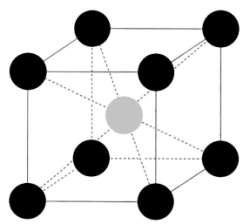
\includegraphics{images/einleitung_hurensohn.jpg}
        \label{einleitung}
        \caption{Basiszelle Cu$_3$Au}
    \end{figure}  
   
\section{Theoretische Vorbereitung}
    \subsection{Reziprokes Gitter}
        Das reziproke Gitter beschreibt in der Festkörperphysik die Röntgen-, Elektronen-, und Neutronenbeugung
        an Kristallinen strukturen. Es wird häufig in zusammenhang mit den Miller'schen Indizes verwendet
        um die Netebenen $(hkl)$ zu beschreiben. Es bietet sich an diese im Reziproken zu definieren, da die Länge
        eines Vektors der die Position eines Gitterpunkts beschreibt gleich dem Reziproken des Abstands der
        Netzebenen entspricht.
        Aus den Basisvektoren des Punktgitter ($\vec{a_1},\vec{a_2},\vec{a_3}$) ergeben sich über folgende Beziehung
        die Basisvektoren ($\vec{b_1},\vec{b_2},\vec{b_3}$) des Reziproken gitters.
        \begin{align*}
            \vec{b_1} = 2\pi \frac{\vec{a_2}\times \vec{a_3}}{\vec{a_1}\cdot (\vec{a_2}\times \vec{a_3})}
            \\\vec{b_2} = 2\pi \frac{\vec{a_3}\times \vec{a_1}}{\vec{a_1}\cdot (\vec{a_2}\times \vec{a_3})}
            \\\vec{b_3} = 2\pi \frac{\vec{a_1}\times \vec{a_2}}{\vec{a_1}\cdot (\vec{a_2}\times \vec{a_3})}
        \end{align*}
        Über diese Definition der Basisvektoren lassen sich die Koordinaten eines Punktes im reziproken Gitter
        über die Miller'schen indizes $(hkl)$ beschreiben.
        
        \subsubsection*{Bragg Gleichung}
            Die Bragg Gleichung liefert einen Zusammenhang zwischen dem Netzebenenabstand $d_{hkl}$ und dem
            Beugungswinkel $\theta$. Damit dieser Zusammenhang gilt muss jedoch der einfallende und gestreute
            Strahl symetrisch zur reflektierende Netzebene verlaufen. Dann lässt sich der Zusammenhang beschreiben durch
            \begin{equation}
                n\lambda = 2d_{hkl} \sin(\theta)
            \end{equation}
            aus dieser lässt sich die äquivalente Laue Bedingung ableiten, welche aussagt,
            dass ein Röntgenstrahl genau dann gestreut wird, wenn der Beugungsvektor $\vec{k}$ gleich dem
            reziproken Gittervektor ist. 
    
    \subsection{Ordnungsparameter und Phasenübergänge}
       Bei einem Phasenübergang handelt es sich um eine Umwandelung einer Phase eines Stoffes in 
       eine andere Phase. Diese Übergänge treten meist in Abhängigkeit von einem oder mehrerer Zustandsvariablen
       wie Druck oder Temperatur auf.\\
       Will man nun den Zustand eines Physikalischen systems nicht nur vor und nach einem Übergang beschreiben,
       so dienen die Ordnungsparameter zur eben dieser. Geht man beispielsweise von einem Übergang von einer
       flüssigen in eine feste Phase, wie beispielweise bei gefrierung von Wasser, so geht das System von einer
       hohen Symetrie in eine Phase in der lediglich die Gittersymetrie verbleibt. Dieser Übergang lässt sich
       anhand des Ordnungsparameters als Übergang von absoluter Unordnung ($s=0$) zu einer höheren Ordnung
       ($s=c\in \Re^+$) beschreiben. Diese Beschreibung lässt sich auf beliebige Übergänge übertragen, bei denen
       gegebenenfalls kein eindeutiger Phasenwechsel auftritt, ja nach dem verändert sich der Ordnungsparameter
       entweder plötzlich oder kontinuierlich. Anhand der Thermondynamik lässt sich über
       \begin{equation}
           F = E-TS
       \end{equation}
       zeigen, dass der Ordnungsparameter stehts versucht die freie Energie zu minimieren um schlussendlich
       einen Gleichgewichtszustand mit mininmaler freien Energie zu erreichen. 

    \subsection{Überstrukturen}
        Eine Überstruktur beschreibt eine Elementarzelle die größer ist als diejenige die man beim Durchschneiden
        des Kristallgitters erhalten würde. Nimmt man beispielsweise eine reine Oberfläche/Kristalline Struktur an, so
        gäbe es keine Überstrukturen, diese kommen erst dann zustande wenn beispielweise Adsorbatome an einer Oberfläche
        eine weiteres geordnetes Gitter bilden welches größer ist als das des reinen ursprünglichen Gitters.
        Überstrukturen werden nach Wood, über ein vielfaches der reziproken Gittervektoren angegeben, beispielweise
        \begin{align*}
            (2\times1) \text{  die Überstruktur ist in x-Richtung doppelt so groß wie die Elementar Zelle}\\
            (\sqrt{2}\times\sqrt{2})R45 \text{  um 45° rotierte quadratische Zelle}
        \end{align*}
        Überstrukturen lassen sich beispielsweise direkt mit dem Rastertunnelmikroskop sichtbar gemacht werden.
        Andererseits lässt sich über Beugungsverfahren das reziproke Gitter der Oberfläche abbilden, bei der die
        Überstruktur zu zusätzlichen Gitterpunkten im reziproken Gitter in form von zusätzlichen Beugungsmaxima
        führt. 

        \subsection{Legierung}
            Eine Legierung ist ein Gemisch aus mindestens einem Metall (Basismetall) und einem anderen Element (Komponente). Im Allgemeinen 
            haben Legierungen einen kristallinen Aufbau. Die Legierung weisst andere chemische Eigenschaften, wie Härte oder elektrische Leitfähigkeit,
            auf als das Basismetall. Künstliche Legierungen können dazu verwendet werden, um Werkstoffeigenschaften auf gewünschte Weise zu ändern.
        \subsubsection{$CuZn$ - Legierung}
            Die $CuZn$ Legierung (Messing) kristalisiert in einem bcc-Gitter. Beide Elemente kristallisieren in einem sc-Gitter,
            wobei die beiden Gitter so verschoben sind, dass in einer Zelle sich ein Eckatom des anderen Gitters befindet $\Rightarrow$ bcc-Gitter 
            
        \subsubsection{$CuAu$ - Legierung}
            Wird Kupfer und Gold zu gleichen Teilen gemischt, so bildet sich im ungeordneten Fall eine fcc-Struktur. Die Gitterplätze sind gleichermaßen
            mit Kupfer- und Goldatomen besetzt. Bei der geordneten Struktur sind in der $[001]$-Ebene die Gitterplätze abwechselnd von Kupfer- und Goldatomen besetzt.
            Durch diese abwechselnde Besetzung wird das fcc-Gitter verzerrt, so dass $\frac{\vec{a_3}}{\vec{a_1}} = 0.93$ beobachtet wird.

        \subsubsection{$Cu_3Au$ - Legierung}
            Wird nun Kupfer und Gold 3:1 gemischt, entsteht im ungeordneten Fall wieder ein fcc-Gitter, aber diesmal mit anderen Wahrscheinlichkeiten
            (75\% Kupfer-, 25\% Goldatome). Die geordnete Struktur ist nun deutlich komplizierter. Auf den ersten Blick sieht es wie ein fcc-Gitter aus, 
            jedoch zeichnet sich die $Cu_3Au$ Kristallstruktur dadurch aus, dass sowohl Gold als auch Kupfer in sc-Gittern kristallisieren. Somit liegen 
            vier sc-Gitter ineinander. Die Goldatome formen ein sc-Gitter, welches mit den bisherigen fcc-Gitter Eckatomen übereinstimmt.
            Die übrigbleibenden zentrierten Flächenplätze können nun durch  drei sc-Gitter von Kupferatomen beschrieben werden.
    \subsection{Die röntgenographische Methode}

        \subsubsection{Röntgenstrahlung}    
            Röntgenstrahlung gehört zum elektromagnetischen Spektrum. Röntgenstrahlung entspricht einer Energie von etwa
            100eV oder einer Wellenlänge $~10 nm$. Es gibt unterschiedliche Möglichkeiten Röntgenstrahlung zu erzeugen. 
            Durch Elektronen kann Röntgenstrahlung erzeugt werden, bei hochenergetischen Elektronen Übergängen in Atomen. 
            Bei starkem Beschleunigen (meist Abbremsen oder umlenken) von Elektronen entsteht die sogenannte Bremsstrahlung, welche im Energiebereich
            von Röntgenstrahlung liegt. Somit lässt sich Röntgenstrahlung in einer Röntgenröhre ohne großen Aufwand erzeugen.
            Eine Röntgenröhre besteht aus einer evakuierten Röhre, einer Glükathode und einer Anode. Bei der Glühkathode werden
            freie Elektronen erzeugt und durch einen Spannungsunterschied zur Anode hinbeschleunigt. Beim Auftreffen auf die Anode
            der Elektronen entsteht Röntgenstrahlung. Die erzeugte Röntgenstrahlung besteht aus zwei Komponenten, dem kontinuierlichen Spektrum
            und einem diskreten Linienspektrum. Das kontinuierliche Spektrum wird erzeugt, durch die verschiedenen Endenergien der auftreffenden Elektronen. 
            Das diskrete Linienspektrum entsteht durch das Material der Anode. Wenn die auftreffenden Elektronen die richtige Energie haben, 
            können diese die Atome der Anode anregen, welche wiederum Röntgenstrahlung emittieren.

        \subsubsection{Aufbau eines Röntgendiffraktometers}   
            Es gibt drei verschiedene Methoden der Röntgendiffraktometrie. Alle drei Methoden bauen auf der Bragg-Bedingung auf.
            \begin{enumerate}
                \item   Laue-Verfahren: Hier wird ein kontinuierliches Röntgenspektrum mit fester Orientierung zu einem Einkristall verwendet. 
                        jede Ebenenschar sucht sich genau die Wellenlänge raus, für die die Bragg-Bedingung bei vorgegebenen Winkel erfüllt ist.
                \item   Drehkristall-Verfahren: In diesem Verfahren wird monochromatische Röntgenstrahlung an einem Einkristall gebeugt. Der Einkristall 
                        wird mit einem Detektor gedreht. Immer wenn bei einer Wellenlänge die Bragg-Bedingung erfüllt ist, tritt ein Beugungsreflex auf.
                \item   Debye-Scherrer-Verfahren: Bei dem Debye-Scherrer-Verfahren wird monochromatische Röntgenstrahlung verwendet. Im Unterschied
                        zum Drehkristall-Verfahren besteht hier unsere Probe aus einem Pulver. In diesem Pulver sind die einzelnen Kristalle in alle möglichen 
                        Richtungen gerichtet. 
            \end{enumerate}

        \subsubsection{Intensität der gestreuten Röntgenstrahlung}
            Die Intensität der Röntgenstrahlen ist proportional zum Betragsquadrat des Formfaktors. 
            \begin{equation}
                I_{hkl} \propto |F|^2 p L_P A_t
            \end{equation}
            mit F = Strukturfaktor, p = Flächenhäufigkeitsfaktor, $L_P$ = Lorentz-Polarisationsfaktor und $A_T$ = Absorptionsfaktor
            Der Strukturfaktor gibt die Streudichte einer Elementarzelle an. Er lässt sich aus der Fouriertransformierten
            der Ladungsverteilung bestimmen.
            \begin{equation}
                F_{hkl} = \sum_i f_i e^{i \vec{G} \cdot \vec{r_i}}
            \end{equation}
            $\vec{r_i}$ ist der Ortsvektor der i-ten Atoms, $f_i$ der Atomformfaktor und G der reziproke Gittervektor des vorliegenden Bravais-Gitters
            Für ein kubisches Gitter vereinfacht sich  die Formel zu:
            \begin{equation}
                F_{hkl} = \sum_i f_i e^{i 2 \pi (hx + ky + lz)_i}
            \end{equation}
            Der Lorentz-Polarisationsfaktor ist ein Korrekturterm, welcher die Winkelabhängigkeit der Intensität berücksichtigt. Außerdem,
            dass die beobachteten Peaks keine scharfen Linien bilden.
            \begin{equation}
                L_P = \frac{1 + cos^2(2 \theta)}{sin^2(\theta) cos^2(\theta)}
            \end{equation}

            Eine weitere Korrektur ist der Absorptionsfaktor. Er berücksichtigt die Absorption von Strahlung innerhalb des Materials.
            
        \subsection{Reflexindizierung im Röntgendiffraktogramm}
    
    \subsection{Die resistive Methode}
        Die zweite Methode zur Proben charakterisierung die hier Anwendung findet ist die resistive.
        Dabei erhällt man informationen über die Ordnung s im Kristall über die Messung des Widerstands.
        \subsubsection{Elektrische Leitfähigkeit}
            Möchte man die elektrische Leitung von Elektronen durch ein Metall beschreiben bietet sich unter
            anderem das Modell von Arnold Sommerfeld, auch gennant Drude-Sommerfeld-Modell, an. In diesem Modell
            wird ein elektrischer Leiter mit frei beweglichen Elektronen als Elektronengaß betrachtet.
            Durch ein äußeres Elektrisches Feld erfahren die freien Elektronen im Leiter eine Kraft $F_{el} = qE$
            und es kommt zu einem Stromfluss. Das problem der unbegrenzten Beschleunigung wird durch das Drude-Modell
            durch Stöße zwischen den Elektronen und Gitterionen beschrieben, durch die das Elektron abgebremst wird
            und die Energie als Wärme abgegeben wird. Diese Bewegung lässt sich beschreiben über
            \begin{equation}
                ma + \frac{m}{\tau}v_D = -eE
            \end{equation}  

        \subsubsection{Temperaturabhängigkeit}
            Der speziefische Wiederstand einer Kristallstruktur wie z.B. einer Legierung lässt sich schreiben als
            \begin{equation}
                \rho = \rho_D + \rho_L(T)
            \end{equation}
            wobei $\rho_D$ den sogennanten temperaturunabhängigen Restwiderstand und $\rho_L$ den temperaturabhängigen
            Widerstand beschreibt.\\
            Geht man nun von einem reinen Metall zu einer Legierung ändert sich die Gitterstruktur und 
            damit auch die Defektstellen im ursprünglichen Gitter, wodurch über das Phononenspektrum auch
            die Temperaturabhängigkeit beeinflusst wird. Für kleine Konzentrationen an Fremdatomen ist die
            Zahl der zusätzlichen Defektstellen proportional zur Konzentration. Im falle von $Cu_1-_xAu_x$ ergibt sich
            die folgende quadratische Konzentrationsabhängigkeit für den Restwiderstand
            \begin{equation}
                \rho_D(x) = \rho_D(0)+Ax(1-x)
            \end{equation}  
            mit einer Materialkonstante A.\\
            Für Ordnungsfähige legierungen wie $CuAu$ und $Cu_3Au$ muss zusätzlich noch die Abhängigkeit vom
            Ordnungsgrad $S$ der langreichweitigen Ordnung berücksichtigt werden, da diese ebenfalls ein regelmäßiges
            Gitter bilden.
            \begin{equation}
                \rho_D(x) = \rho_D(0)+Ax(1-x)(1-S^2)
            \end{equation}
            Mit bekanntem Restwiderstand und Materialkonstante lässt sich so der Ordnungsparameter bestimmen.
        
        \subsubsection{Vierpunktmethode}   
            Um nun aus dem Wiederstand den Ordnungsparameter S zu extrahieren lässt sich die Vierpunktmethode
            zur Widerstandsmessung nutzen. Bei dieser werden vier Elektrische Kontakte bzw. Messspitzen auf die 
            Oberfläche gebracht. Nun wird über die äußeren Kontakte ein bekannter/messbarer Strom auf die Oberfläche
            geführt wodurch sich im Material ein Elektrisches Feld ausbildet, welches sich in Form einer 
            Potentialdifferenz aus den mittleren Spitzen bestimmen lässt.
            Wichtig bei dieser Messung ist es möglichst weit von den Rändern der Probe entfernt zu sein, da durch die Randbedingungen der
            Strom dort stehts parralel zum Rand fließt. Im falle der idealisierten annahme und vier Messspitzen 
            mit gleichem Abstand erhält man den Flächenwiderstand $R_{sq}$ über
            \begin{equation}
                R_{sq} = \frac{\pi}{ln2}\frac{U}{I}
            \end{equation}
            wobei U die Potentialdifferenz der Mittleren SPitzen und I der Strom der äusseren Spitzen ist.
            Aus dem Flächenwiderstand lässt sich nun der gewünschte spezifische Widerstand berechnen
            \begin{equation}
                \rho = d R_{sq}
            \end{equation}
            mit d als Schichtdicke der Probe.
  

%\section{Vorbereitende Aufgaben}

 %       \begin{equation}
 %           \theta = \arctan{\frac{b}{d}} = \arctan{\frac{a}{d \sqrt{2}}}
 %       \end{equation}


%    \subsection{1234}
%        \hl{Unterschied zwischen Axialem Druck und Nadeleindruck}

	
%\section{Versuchsaufbau}
    \begin{figure}[ht]
        \centering
        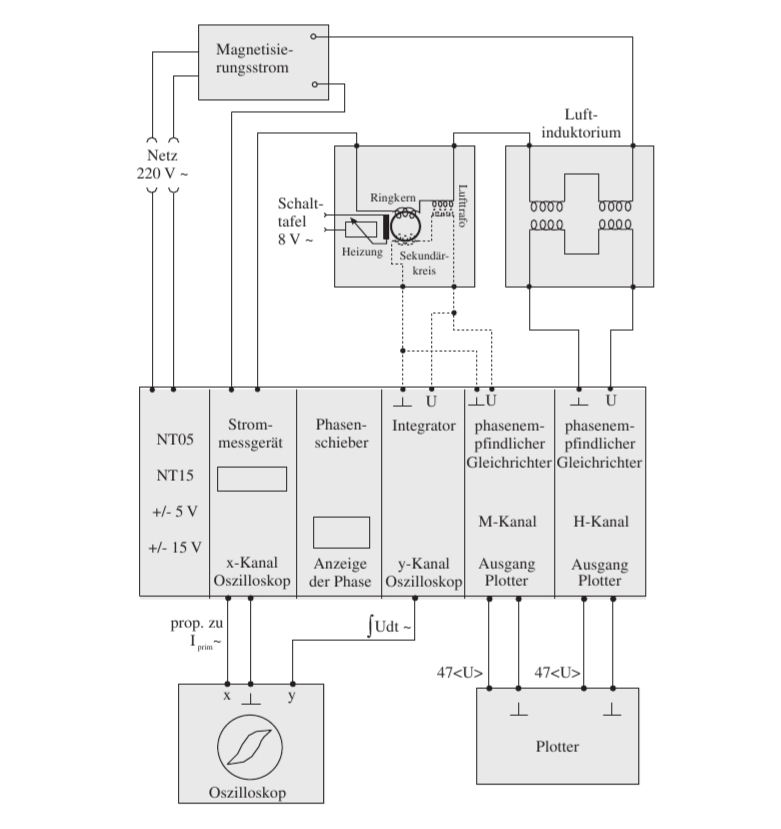
\includegraphics[width=\textwidth]{Images/Schaltplan.PNG}
        \label{Schaltplan}
        \caption{Schaltplan des Versuchs}
    \end{figure}
    Um in diesem Versuch möglichst viele Parameter variieren zu können werden zwei verschiedene Versuchsaufbauten verwendet.

    \subsubsection*{Ringkern mit Heizung}
        Bei diesem Aufbau handelt es sich um einen geschlossenen Ferrit Ringkern mit Heizspule um den Temperaturverlauf aufzeichnen zu können.\\
        Primär- und Sekundärspule haben jeweils $n=17$ Windungen, der Ringkern hat einen Querschnitt von $q=0,9cm^2$ und einen Radius von $r=1.5cm$.
        Die Heizgeschwindigkeit lässt sich über ein Potentiometer regulieren und mit Hilfe eines Thermoelements messen.
    
    \subsection*{Ringkern mit Spalt}
        Um nun im Ringkern einen Spalt zu erzeugen lässt sich dieser Aufbau auseinanderziehen und mit Plättchen variierender Dicke auf vorgegebenen Abständen halten.
        In diesem Aufbau hatte die Primärspule hingegen $n_p=54$ und die Sekundärspule $n_s=17$ Windungen\\
        
    Bei beiden aufbauten wurde, um den Einfluss der Umgebung zu eliminieren, je ein Luftinduktor in Reihe geschaltet. Die Messausgänge der Gesamtschaltung (siehe \ref{Schaltplan}) konnten 
    dabei je nach Messung zwischen den Eingängen des Oszilloskops und der Gleichrichter gewechselt werden. 

\include{Chapters/Durchführung.tex}

\section{Auswertung}
	Da unsere getemperte Probe ungewöhnlich viele Ätzgrübchen aufweist und im Verlauf des Versuchs beschädigt wurde, haben wir eine weitere getemperte Probe erhalten und somit insgesamt 3 Proben untersucht.
    \subsection{Ätzgrübchendichte}
        Zunächst gilt es, als eine erste Näherung der Versetzungsdichte die Ätzgrübchendichte an der Oberfläche zu bestimmen.
	Dazu wurden für beide Proben je 3 Bilder von verschiedenen Positionen an der Oberfläche aufgenommen und anschließend
        aus der Fläche, aufgenommen durch das Mikroskop, und den sichtbaren Ätzgrübchen die Ätzgrübchendichte bestimmt. Dieser Vorgang ist,
        durch das manuelle Zählen der Grübchen sehr müßig und ungenau, lässt aber dennoch eine Qualitative aussage über die Ordnung im Kristall zu.
        Aus den Aufgenommen Bildern lies sich folgende Tabelle erstellen.
        \begin{table}[H]
            \centering
            \begin{tabular}[]{c|c|c|c|c}
                Probe & Aufnahme Nr. & Anzahl Grübchen & Fläche [$\mu m^2$] & Dichte [$\frac{n}{\mu m^2}$] \\
                \hline
                \multirow{3}{*}{\rotatebox[origin=c]{90}{Get.}} & 1 & $39 \pm 3$ & 839908,67$\pm$0,01 & $(4,64\pm 0,37)\cdot 10^{-5}$ \\
                                                                     & 2 & $25 \pm 3$ & 1099357,61$\pm$0,01 & $(2,27\pm 0,28)\cdot 10^{-5}$ \\
                                                                     & 3 & $31 \pm 3$ & 454314,66$\pm$0,01 & $(6,82\pm 0,67)\cdot 10^{-5}$ \\
                Mittelwert                                           & - & - & - & $(4,6\pm 0,47)\cdot 10^{e-5}$\\
                \hline
                \multirow{3}{*}{\rotatebox[origin=c]{90}{Unget.}}  & 1 & $344 \pm 40$  & 18894,73$\pm$0,01 & $(1,82 \pm 0,21)\cdot 10^{-2}$ \\
                                                                        & 2 & $27 \pm 5$    & 7942,73$\pm$0,01 & $(0,34\pm 0,06)\cdot 10^{-2}$ \\
                                                                        & 3 & $103 \pm 15$  & 6251,25$\pm$0,01 & $(1,74e\pm 0,24)\cdot 10^{-2}$ \\
                Mittelwert                                           & - & - & - & $(1,27 \pm 0,19)\cdot 10^{-2}$\\
                
            \end{tabular}    
        \end{table}
	Als Flächenfehler nehmen wir an, dass aus der angegebenen Genauigkeit des Auswertungsprogramms ein Fehler von 0,1 $\mu m^2$ resultiert.
	Der Fehler der Dichte ergibt sich gemäß Fortpflanzung zu $\Delta \rho = \sqrt{(\frac{\Delta n}{A})^2 + (\frac{n\Delta A}{A^2})^2}$.
	Den Gesamtfehler des Mittelwerts bestimmen wir über $\Delta \rho^2 = (\sum_{i=1}^3 \Delta \rho_i^2)/3$, mit den drei Einzelfehlern $\rho_i$. Die Standardabweichung zum Mittelwert der getemperten Probe beträgt $2,27\cdot 10^{-2}$, der Standardfehler $1,31\cdot 10^{-5}$, diese Werte berücksichtigen jedoch keine Grübchenzahl- und Flächenfehler. Für die ungetemperte Probe ergeben sich eine Standardabweichung von $0,8\cdot 10^{-2}$ sowie ein Standardfehler von $0,5\cdot 10^{-2}$.\\
        Es ist deutlich zu erkennen, dass die Ätzgrübchendichte der ungetemperten Probe um ein Vielfaches höher ist, als die der getemperten.
        Auch ist zu erkennen, dass die Ätzgrübchendichte an verschiedenen stellen der Oberfläche stark variiert, also nicht konstant ist.
    \begin{figure}[H]
        \centering
        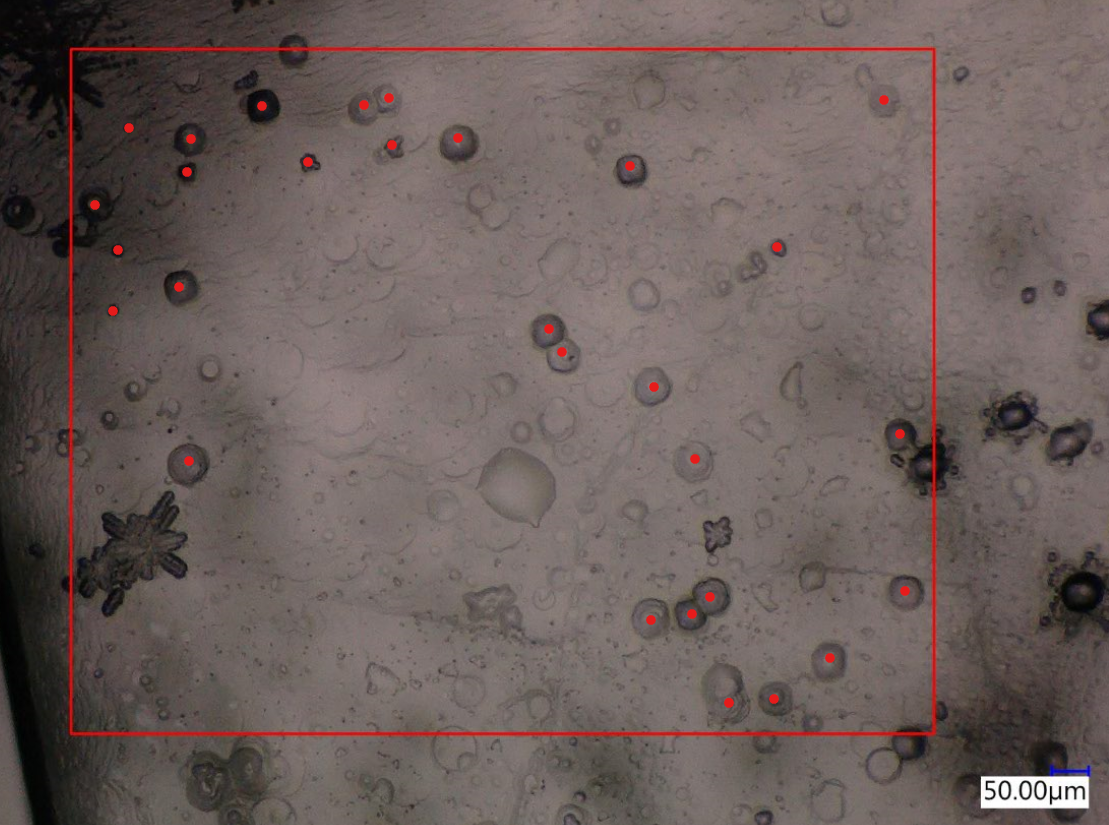
\includegraphics[width=\textwidth]{Images/Beispiel_ätzgrübchendichte.PNG}
        \caption{Beispiel einer Aufnahme für die Ätzgrübchendichte.}
    \end{figure}

    \subsection{Kleinwinkelkorngrenzen}
        \subsubsection*{Rosetten durch Nadeleindruck}
            Im Anschluss an die Bestimmung der Ätzgrübchendichte wurde auch ein Bild einer vermutlichen Kleinwinkelkorngrenzen aufgenommen, um aus diesem
            den Winkel zwischen den Kristalliten zu bestimmen. Um den Winkel aus den Abständen zwischen den Ätzgrübchen zu bestimmen wurde bereits in der Vorbereitung
            folgende Formel hergeleitet
            \begin{equation}
                \theta \approx \frac{b}{d} \approx \frac{(n-1)\cdot a}{\sqrt{2}\cdot d}
            \end{equation}
            Wobei $n$ die Anzahl der Ätzgrübchen angibt und $d$ den abstand zwischen dem ersten und letzten. Zudem nehmen wir für $b=\frac{a}{\sqrt{2}}$ an, sodass für
            Messungen mit mehreren Grübchen ein gesamt Verschiebung von $b_ges = n * g$ gilt.
            Mit folgender Aufnahme
            \begin{figure}[H]
                \centering
                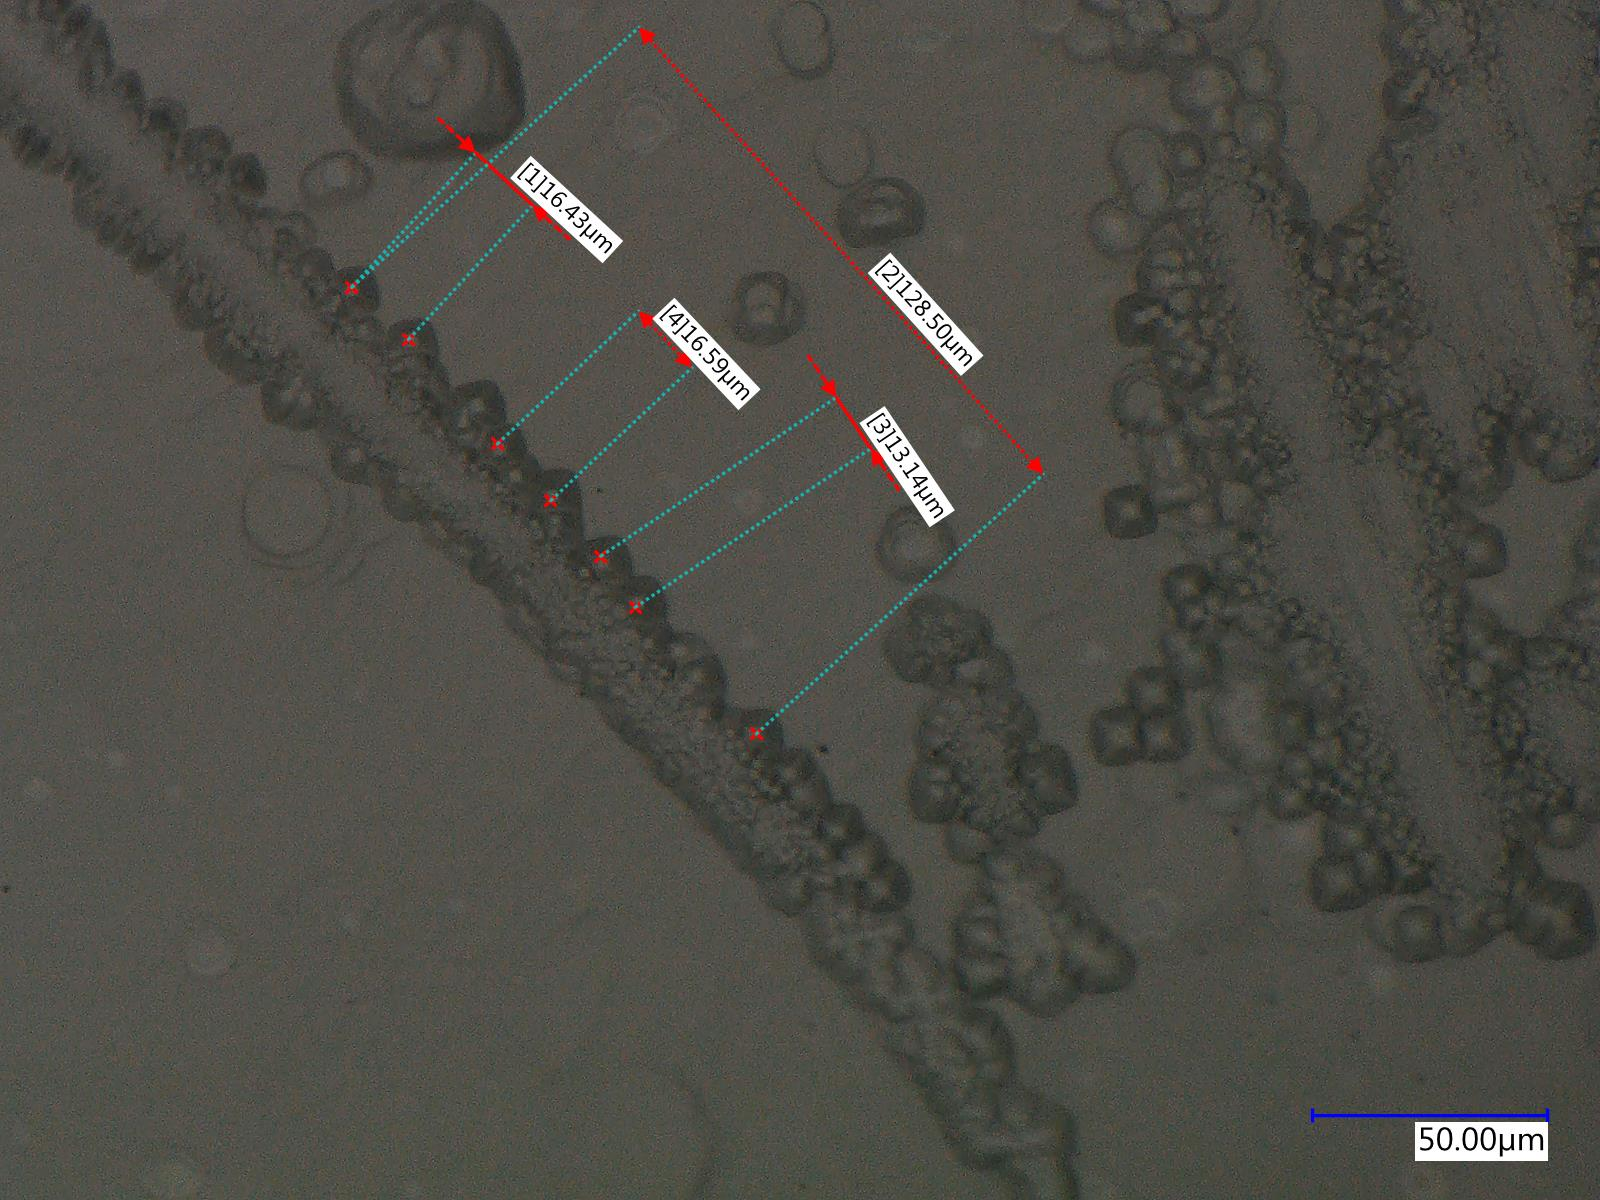
\includegraphics[width=\textwidth]{Images/kleinwinkelkorngrenze 2.jpg}
                \caption{Aufnahme einer vermutlichen Kleinwinkelkorngrenzen mit Abständen}
            \end{figure}
            konnte folgende Tabelle erstellt werden
            \begin{table}[H]
                \centering
                \begin{tabular}[]{c|c|c}
                    Abstand d [$\mu m$] & Anzahl Grübchen (n-1) & Winkel $\theta$ [°] \\
                    \hline
                    $128,5 \pm 0.1$ & 9 & $(1,14 \pm 0,0192)\cdot 10^{-3}$\\
                    $16,4 \pm 0.1$ & 1 & $(0,99 \pm 0,151)\cdot 10^{-3}$\\
                    $16,6 \pm 0.1$ & 2 & $(1,96 \pm 0,149)\cdot 10^{-3}$\\
                    $13,1 \pm 0.1$ & 1 & $(1,24 \pm 0,189)\cdot 10^{-3}$\\   
                \end{tabular}
            \end{table}
		Die jeweiligen Winkelfehler ergeben sich dabei durch Fehlerfortpflanzung aus $\Delta \theta = \frac{(n-1)\cdot a}{\theta\cdot d^2}\cdot \Delta d$.
            Grundsätzlich entsprechen die Winkel den Erwartungen, da diese recht klein ausfallen. Eine Kleinwinkelkorngrenze, die mehr auf einer Linie befindliche Ätzgrübchen erzeugt hätte,
		hätte jedoch eine genauere Winkelmessung ermöglicht.
% jedoch lässt die Messmethode nur ganzzahlige n zu, die nur eine geringe Auflösung der Tatsächlichen abstände d zulassen.
        \subsection{Versetzungsbewegungen}
            Dieser abschnitt befasst sich mit der Wanderung der Versetzungen bei äußerer Druckeinwirkung, dazu wurden 2-3 Rosetten durch Nadeleindruck erzeugt,
            deren Dimension über das Mikroskop aufgenommen und anschließend durch axialen Druck bewegt. Durch das Gewicht der Presse sowie der Querschnittsfläche der Probe
            lässt sich die Kraft bestimmen und über die Dauer der Anwendung die Geschwindigkeit der Wanderung.
            \begin{figure}[H]
                \begin{minipage}[b]{.4\linewidth} % [b] => Ausrichtung an \caption
                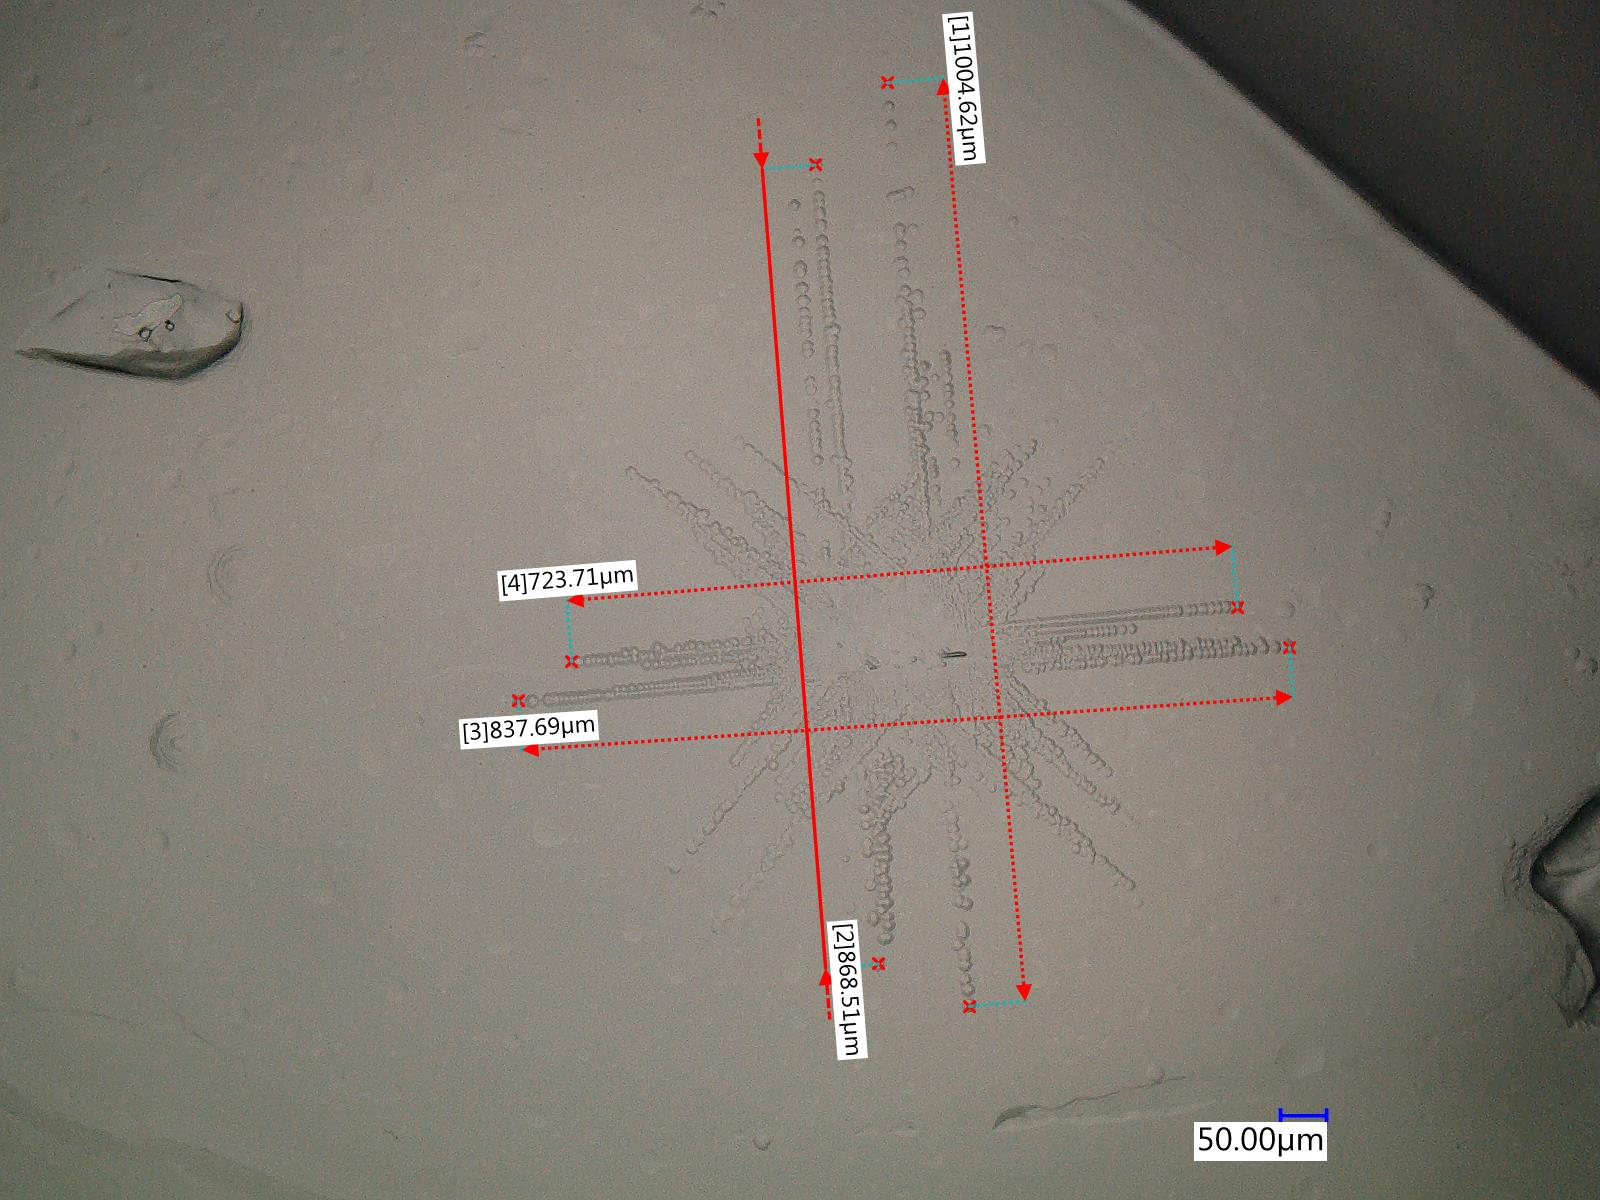
\includegraphics[width=\linewidth]{Images/eriks rosette 1 messung A.jpg}
                \end{minipage}
                \hspace{.1\linewidth}% Abstand zwischen Bilder
                \begin{minipage}[b]{.4\linewidth} % [b] => Ausrichtung an \caption
                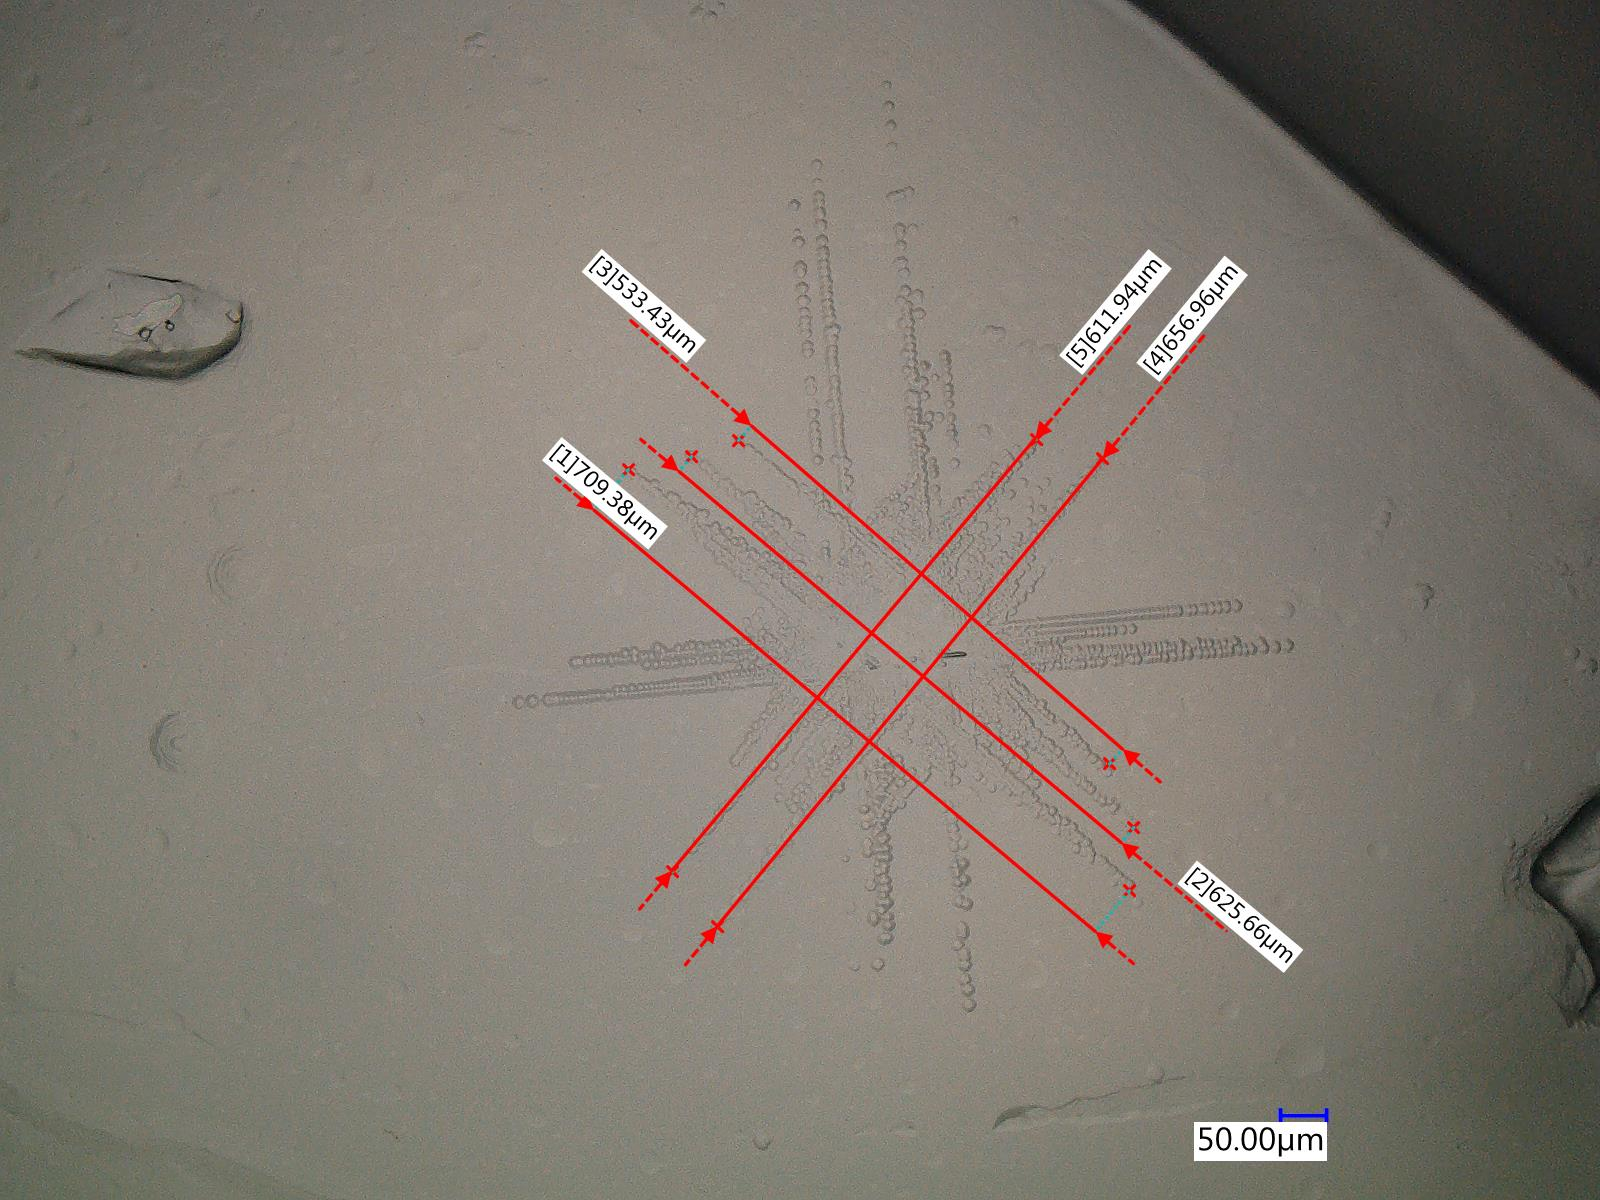
\includegraphics[width=\linewidth]{Images/eriks rosette 1 messung B.jpg}
                \end{minipage}
                \caption{Aufnahme eines Nadeleindrucks mit Abmessungen vor der Anwendung des Axialen Drucks}
            \end{figure}
            \begin{figure}[H]
                \centering
                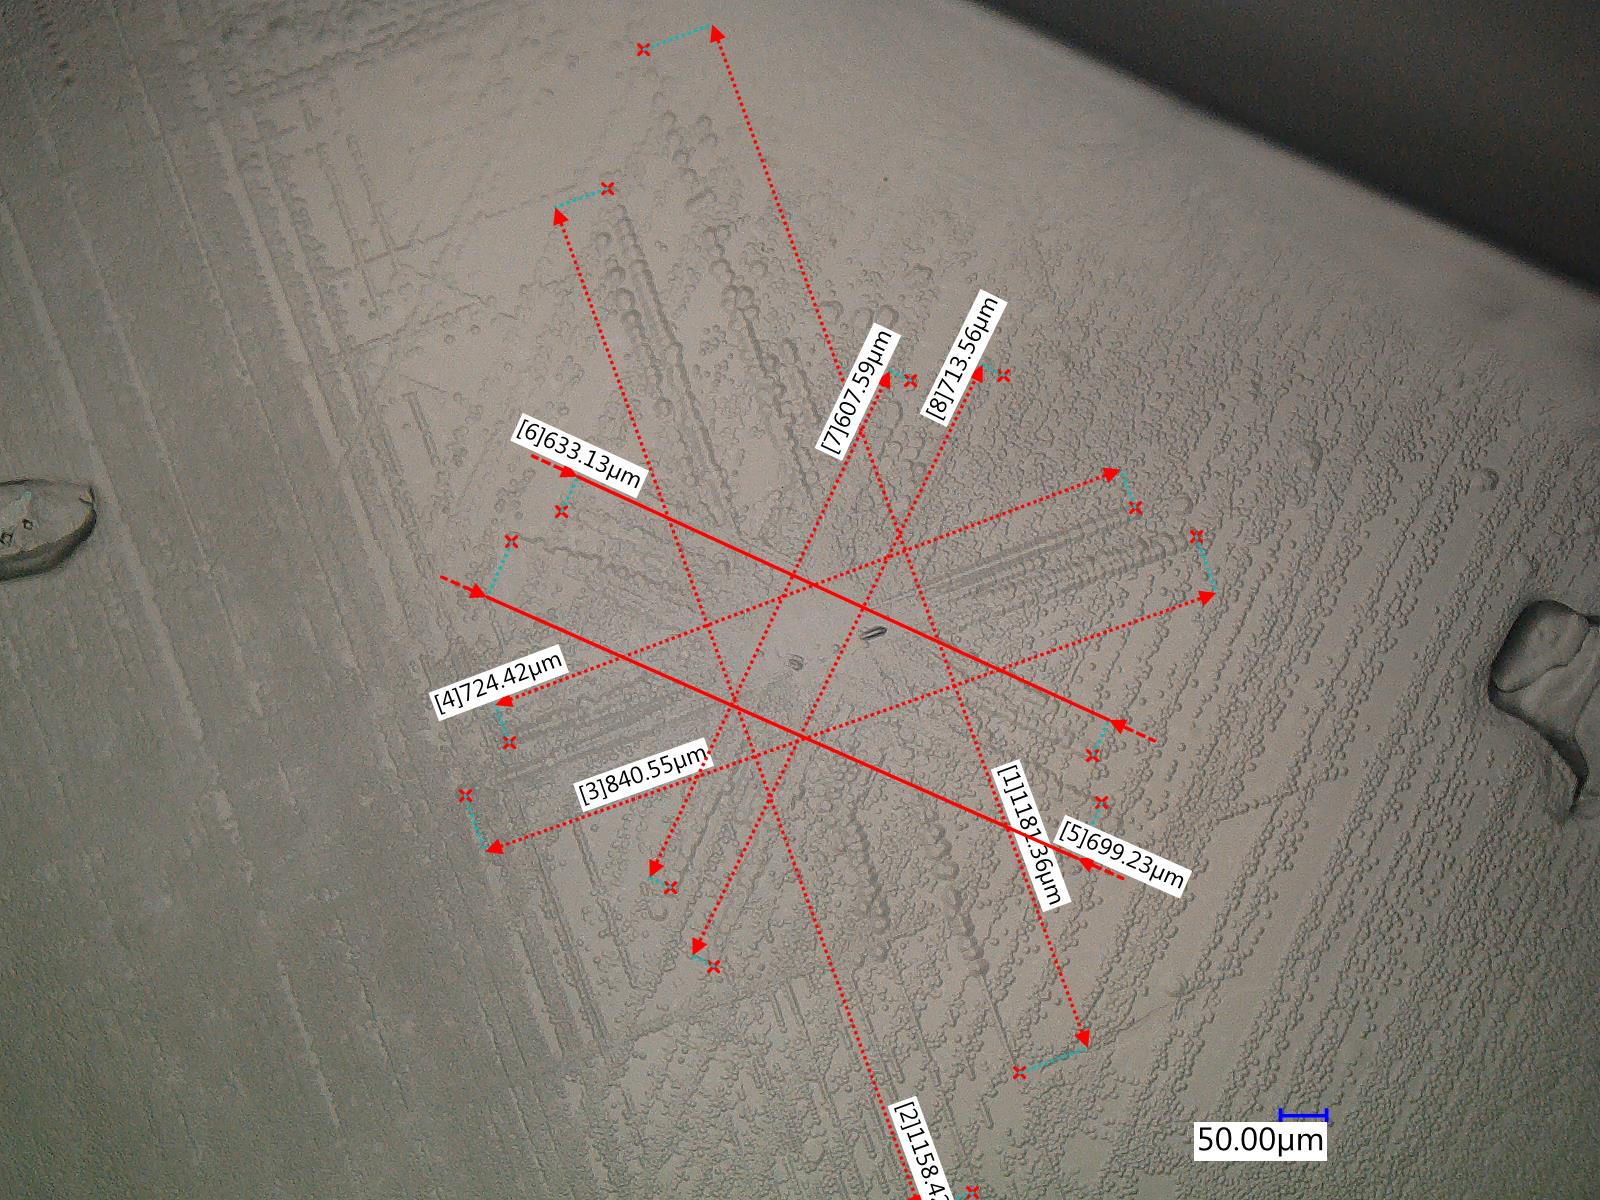
\includegraphics[width=\linewidth]{Images/eriks rosette 1PD Messung.jpg}
                \caption{Aufnahme eines Nadeleindrucks mit Abmessungen nach der Anwendung des Axialen Drucks}
            \end{figure}
            Aus den Messungen durch das Mikroskop lassen sich grob folgende Messungen für die Wanderungsdistanz bestimmen
            \begin{table}[H]
                \centering
                \begin{tabular}[]{c|c|c|c}
                    Vorher [$\mu m$] & Nachher [$\mu m$] & Differenz [$\mu m$] & Geschwindigkeit [$\frac{\mu m}{min}$] \\
                    \hline
                    $838 \pm 5$  & $841 \pm 5$    & $ 3 \pm 10$     & $1,0 \pm 3,3$ \\
                    $724 \pm 5$  & $724 \pm 5$    & $ 1 \pm 10$    & $0,2 \pm 3,3$ \\
                    $869 \pm 5$  & $1158 \pm 5$   & $ 290 \pm 10$  & $96,6 \pm 8,7$\\
                    $1005 \pm 5$ & $1181 \pm 5$   & $ 177 \pm 10$  & $58,9 \pm 5,9$\\
                    $533 \pm 5$  & $633 \pm 5$    & $ 100 \pm 10$    & $33,2 \pm 4,3$\\
                    $709 \pm 5$  & $699 \pm 5$    & $ -10 \pm 10$  & $-3,4 \pm 3,4$\\
                    $612 \pm 5$  & $608 \pm 5$    & $ -4 \pm 10$   & $-1,5 \pm 3,3$\\
                    $657  \pm 5$ & $714  \pm 5$   & $ 57 \pm 10$    & $18,9 \pm 3,7$\\
                \end{tabular}
                \caption{Messung der Wanderung der Rosettenarme}
            \end{table}
            Es ist deutlich zu erkennen, dass durch den axialen Druck nur wenige Arme entlang der $<110>$ - Richtung ein Starkes Wachstum erfahren haben, das Wachstum der anderen Arme ist im Rahmen unserer
            Messgenauigkeit kaum aussagekräftig, ließe sich jedoch auf die statistische Verteilung der Energie entlang aller Achsen zurückführen.
		Das ausbleibende Wachstum der Arme in $<100>$ - Richtung entspricht grundsätzlich unseren Erwartungen, wir hätten allerdings auch ein deutlicher sichtbares Wachstum der Arme in $<110>$ - Richtung erwartet.
		Vermutlich hätte sich durch ein höheres Lastgewicht oder eine erhöhte Belastungsdauer ein stärkeres Wachstum ergeben. Genauso hätte dies jedoch auch eine Zunahme der Fehlstellen abseits der Nadeleindrücke
		verursachen können, was die Auswertung an dieser Stelle erschwert hätte. Bereits in unserer Aufnahme ist zu erkennen, dass sich durch die Belastung unzählige zusätzliche Fehlstellen auf der Kristalloberfläche
		gebildet haben.
        \subsubsection*{Schubspannung im Gleitsystem}
            Um den Druck im Gleitsystem zu bestimmen wurde das angewandte Gewicht ($m = 2,716\pm0,01\text{ Kg}$) der Presse sowie die Druckfläche ($A=3618962\text{ }\mu m^2$)der Probe bestimmt.
            Mit
            \begin{equation}
                F = m \cdot a = 26,64\pm0,10\text{ N}
            \end{equation}
            folgt die Kraft (Fehler: 0,01 Kg$\cdot$9,81 m/s$^2 \approx$ 0,10). Die Kraft entlang der bevorzugten 
            gleitebene berechnet sich mit der Gitterkonstante a=0.402 nm zu\cite{7} 
            \begin{equation}
                F_{<110>} = F\cdot b_{<110>}^2 = \frac{a^2}{2} \cdot F 
            \end{equation}
            und anschließend die über
            \begin{equation}
                \sigma = F_{<110>} \cos{(\pi / 4)}/ A = (4,2 \pm 0,016)\cdot 10^{-13}\text{ }\frac{N}{m}
            \end{equation}
            die Schubspannung. Der Fehler ergibt sich unter der Annahme, dass unsere Auswahl der Messpunkte im Auswertungsprogramm des Mikroskops eine lineare Ungenauigkeit von 1$\mu$m (und somit einen Flächenfehler von (1$\mu$m)$^2$) aufweist, mittels Fehlerfortpflanzung aus $\Delta \sigma^2 = (\frac{\cos{(\pi / 4)} \Delta F_{<110>}}{A})^2 + ( \frac{\cos{(\pi / 4)} F_{<110>} \Delta A}{A^2})^2$.

\section{Diskussion}
    Abschließend noch eine Zusammenfassung des Versuchs und eine Diskussion
    unserer Ergebnisse.
    Ziel des Versuchs war es, von drei Proben von Cu$_3$Au mit einem
    unterschiedlichen Ordnungsgrad, diesen zu bestimmen. 
    Dies wurde mit zwei verschiedenen Messmethoden erreicht: 
    \begin{itemize}
        \item Der Röntgendiffraktometrie
        \item dem resistiven Verfahren
    \end{itemize}
    Bei der Röntgendiffraktometrie wurde sich die Bragg-Bedingung zunutze gemacht
    indem man die Fundamentalreflexe mit den Überstrukturreflexen verglichen und 
    daraus der Ordnungsgrad bestimmen konnte, sowie auch die Gitterkonstante
    von Cu$_3$Au. Bei dem resistiven Verfahren wurden die Ordnungsgrade 
    durch Widerstandsmessung bei kleinen Temperaturen bestimmt.

    Unsere Ergebnisse für die Gitterkonstanten der 3 Proben $\bar{a}_{Probe2} = (3,74 \pm 0,002)[\mathring{A}]$,
    $\bar{a}_{Probe3} = (3,77 \pm 0,006)[\mathring{A}]$ und $\bar{a}_{Probe4} = (3,86 \pm 0,001)[\mathring{A}]$ liegen
    alle nicht im Fehlerbereich des Literaturwerts: $a_{Cu_3Au} = 3.7490\mathring{A}$ \footnote{http://som.web.cmu.edu/structures/S005-Cu3Au.html}
    jedoch ist eine Abweichung von 0,2 \% sehr gut (Probe 2), bei Probe 4 ist die Abweichung schon 3\%, was aber 
    auch noch sehr zufriedenstellend ist. Eine mögliche Abweichung der Proben könnte aus der Annahme der perfekten Ordnung und der kubischen Gitterstruktur kommen. Außerdem war es schwierig und relativ ungenau die Überstrukturpeaks zu bestimmen und zu fitten.
    Die Fundamentalreflexe waren bei jeder Probe deutlich ausgeprägt und leicht zu identifizieren, die Überstrukturpeaks 
    waren jedoch teilweise kaum vom Rauschen zu unterscheiden.
    
    Bei der Bestimmung des Ordnungsgrades der beiden Proben mit der röntgenographischen Methode kam heraus, 
    dass Probe 2 um ca. 18\% geordneter ist, als Probe 3. Jedoch ist der Fehler des Ordnungsgrades von Probe 3 sehr groß ($S_3= 0.39\pm 0.22$).
    Dieser große Fehler wird durch den einen fehlerhaften Messwert bzw. errechneten Ordnungsgrad $>1$ verursacht.
    Eine mögliche Erklärung für diesen Wert ist, wie oben schon beschrieben, die schwer zu erkennenden Überstrukturpeaks.
    Dass Probe 4 vollständig ungeordnet ist, war schon klar als nur die Fundamentalreflexe aufgetreten sind. Dies wurde
    auch bei der resistiven Methode erkannt. Insgesamt sind die Ergebnisse der röntgenographischen Methode
    zufriedenstellend genau.

    Bei der Auswertung der resistiven Methode haben wir angenommen, dass die Probe 4 vollständig
    ungeordnet und die Probe 2 vollständig geordnet ist. Dadruch konnten wir dann, durch umstellen einiger Formeln
    auf einen Ordnungsgrad der Probe 3 von $S_{Probe 3} = 0.997 \pm 0.018$ errechnen. 
    Dies würde einer Probe, welche nahezu vollständig geordnet ist, entsprechen. 
    Der Literaturwert für den spezifischen Widerstand einer geordneten Cu$_3$Au Probe beträgt: $4.2 \cdot 10^{-8}\Omega$, von einer ungeordneten
    Probe: $11,4\cdot 10^{-8}\Omega$ \footnote{https://onlinelibrary.wiley.com/doi/epdf/10.1002/andp.19334100504}.
    Unser errechneten Werte der spezifischen Widerstände weichen um einiges an dem Literaturwert ab.
    Probe 2 um 40\%, Probe 3 um 50\% und Probe 4 um 70\%. Diese Abweichungen lassen sich durch 
    unsere vorher getroffenen Annahmen erklären. Anscheinend sind weder Probe 2 noch Probe 4 vollständig geordnet bzw. ungeordnet.
    Dies ist eine mögliche Fehlerquelle, auch für unsere Bestimmung des Ordnungsgrades.
    
    Alles in allem lässt sich sagen, dass wir nur für die Probe 4 feststellen konnten, dass diese vollständig ungeordnet sein muss
    (nur Fundamentalreflexe und größter Widerstand). Für die Proben 2 und 3 konnten wir jedoch keine wirklich zufriedenstellende
    Ordnungsgrade bestimmen. Laut Versuchsteil 1 sind die Proben weder vollständig geordnet noch ungeordnet, sondern in einem
    Zwischenzustand. In Versuchsteil 2 jedoch nehmen wir Probe 2 als vollständig geordnet an und bestimmen
    dann einen Ordnungsgrad von $0.997$ für Probe 3, was nahezu vollständig geordnet entspricht. 
    Unsere bestimmten Gitterkonstanten sind jedoch sehr genau und sehr zufriedenstellend.

\begin{thebibliography}{9}
	\bibitem{1}
		https://www.princeton.edu/$\sim$maelabs/mae324/glos324/y58-1.gif
	\bibitem{2}
		https://docplayer.org/docs-images/74/70315204/images/31-0.jpg
	\bibitem{3}
		http://muenchuwe.com/nonhtml/papers/fest-25.pdf
	\bibitem{4}
		https://www.ahoefler.de/index.php?option=com\_content\&view=article\&id=294:2-dimensionale-gitterdefekte\&catid=90:gitterdefekte\&lang=de-de
	\bibitem{5}
		https://physik.cosmos-indirekt.de/Physik-Schule/Versetzung\_(Materialwissenschaft)
	\bibitem{6}
		https://de.wikipedia.org/wiki/Lithiumfluorid
\end{thebibliography}

\end{document}